\chapter{提案手法}
\label{chap:method}

3章では、自身の研究で提案する具体的な手法について説明していく。
研究の中身がどのような内容か、自分の意見や考察を書くというわけでなく、「ファクト(事実)」をそのまま書くだけなので、研究全体の中では、もっとも書き進めやすい部分となる。
執筆できるところは研究を進めながらまとめてしまうとよいし、論文全体の中でも先に書き始めてしまってもよい。

手法の説明冒頭では、できるだけ全体像を示すとよい。
図などを使って、必要な構成要素などを列挙しておいて、それを説明する形にすると執筆が進めやすい。

本研究の提案手法の概要を図\ref{fig:overview}に示す。

\begin{figure}[htb]
    \centering
    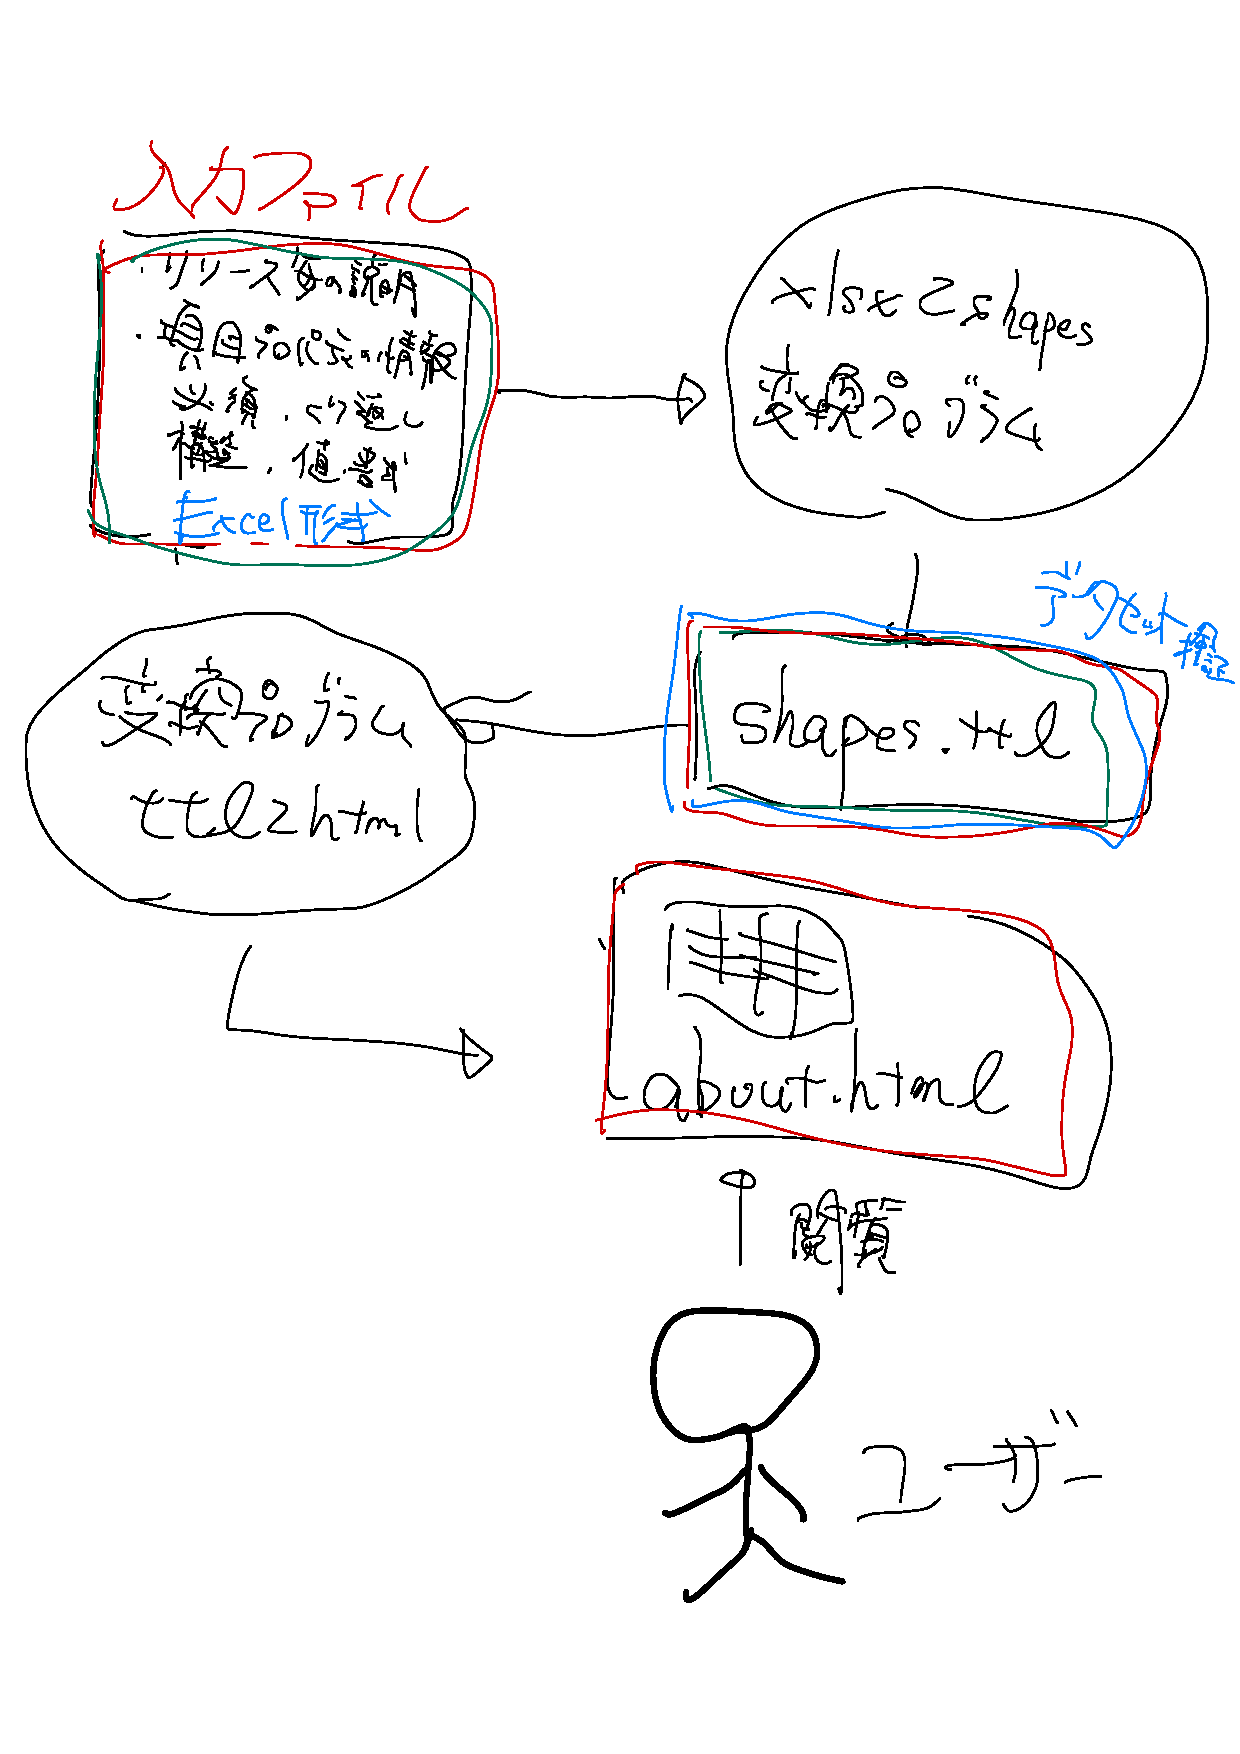
\includegraphics[width=.4\hsize]{figures/overview.pdf}
    \caption{提案手法の概要}
    \label{fig:overview}
\end{figure}

なお、図中における同じカテゴリの要素は、形や色などで同一であることがわかるように区別して示すとよい。
逆に、別のカテゴリの要素を同じような形で書くと紛らわしいので注意する。
図\ref{fig:overview}では、入出力ファイルが四角形、処理プログラムが楕円形で表現されている。

さらなる詳細は、以下のように、全体の処理の流れや構成要素ごとに、節に分けて詳細を説明する。

\section{サブシステムA}

必要に応じて、サブシステムや構成要素ごとに細分化された構成要素をさらに解説する。

\section{サブシステムB}
